%%%% using 'arara' 4.0
% arara: xelatex: {synctex: yes, interaction: nonstopmode}
% arara: bibtex
% arara: xelatex: {synctex: yes, interaction: nonstopmode}
% arara: xelatex: {synctex: yes, interaction: nonstopmode}

% arara: indent: {overwrite: yes}

% arara: clean: { extensions: [aux, bcf, cod, blg, lof, lot, out, toc, log, xml, bak0 ] }

\documentclass[review]{elsarticle}

% Figures Links, mittig und rechts platzieren
\usepackage[export]{adjustbox}
\usepackage{caption}
\usepackage{subcaption}
\usepackage{amsmath}

\usepackage{enumerate}

% prevents that appendices are moved behind references
\usepackage{placeins}

\usepackage[nolist]{acronym}

\usepackage{longtable}
\usepackage{booktabs}
\usepackage{multirow}
\usepackage{float}

% https://tex.stackexchange.com/questions/165115/getting-not-defining-perthousnad-and-not-defining-micro-when-compiling-beamer
\usepackage{textcomp}

\graphicspath{{../03_figures/results/}{./}{../03_figures/data/}} 

% enable paragraph as 4th level https://tex.stackexchange.com/questions/60209/how-to-add-an-extra-level-of-sections-with-headings-below-subsubsection
\usepackage{titlesec}
\setcounter{secnumdepth}{4}
\titleformat{\paragraph}
{\normalfont\small\bfseries}{\theparagraph}{1em}{}
\titlespacing*{\paragraph}
{0pt}{3.25ex plus 1ex minus .2ex}{1.5ex plus .2ex}

% enable linking to subsubsection
\setcounter{secnumdepth}{3}

% various symbols, e.g. \degree
\usepackage{gensymb}

\usepackage[hidelinks]{hyperref}

\usepackage{lineno}
\modulolinenumbers[5]

% set autoref abbr for appendix
\newcommand*{\Appendixautorefname}{appendix}

\journal{Journal "Remote Sensing of Environment"}

% line breaks in table cells
\newcommand{\specialcell}[2][l]{%
  \begin{tabular}[#1]{@{}l@{}}#2\end{tabular}}

% tilde
\newcommand{\mytilde}{\raise.17ex\hbox{$\scriptstyle\mathtt{\sim}$}}

%% APA style
\bibliographystyle{model5-names}\biboptions{authoryear}

\begin{document}

\begin{frontmatter}

	\title{Modeling defoliation as a proxy for tree health: A case study using machine-learning and hyperspectral remote sensing data}

	%% Group authors per affiliation:
	\author[FSU]{Patrick Schratz}
	\cortext[mycorrespondingauthor]{Corresponding author}
	\ead{patrick.schratz@uni-jena.de}

	\author[FSU]{Jannes Muenchow}
	\author[NEIKER]{Eugenia Iturritxa}
	%\author[TUDO]{Jakob Richter}
	\author[FSU]{Alexander Brenning}

	\address[FSU]{Department of Geography, GIScience group, Grietgasse 6, 07743, Jena, Germany}
	%\address[NEIKER]{NEIKER, Granja Modelo –Arkaute, Apdo. 46, 01080 Vitoria-Gasteiz, Arab, Spain}
	%\address[TUDO]{Department of Statistics, TU Dortmund University, Germany}

	\begin{abstract}

	\end{abstract}

	\begin{keyword}
		hyperspectral imagery \sep forest health \sep machine-learning \sep variable importance \sep model comparison
	\end{keyword}

\end{frontmatter}

\linenumbers

% längste Abkürzung steht hier!!! in eckigen Klammern
\begin{acronym}[AUROC]

	% geringerer Zeilenabstand
	%\setlength{\itemsep}{-\parsep}
	\acro{AGB}{Above-Ground Biomass}
	\acro{ANN}{Artificial Neural Network}
	\acro{AUROC}{Area Under the Receiver Operating Characteristics Curve}
	\acro{BRT}{Boosted Regression Trees}
	\acro{CART}{Classification and Regression Trees}
	\acro{CV}{cross-validation}
	\acro{ENM}{Environmental Niche Modeling}
	\acro{FPR}{False Positive Rate}
	\acro{GAM}{Generalized Additive Model}
	\acro{GBM}{Gradient Boosting Machine}
	\acro{GLM}{Generalized Linear Model}
	\acro{ICGC}{Institut Cartografic i Geologic de Catalunya}
	\acro{IQR}{Interquartile Range}
	\acro{MARS}{Multivariate Adaptive Regression Splines}
	\acro{MEM}{Maximum Entropy Model}
	\acro{NDII}{Normalized Difference Infrared Index}
	\acro{NIR}{Near-Infrared}
	\acro{NRI}{Normalized Ratio Index}
	\acro{OLS}{Ordinary Least Squares}
	\acro{LOWESS}{Locally Weighted Scatter Plot Smoothing}
	\acro{PISR}{Potential Incoming Solar Radiation}
	\acro{RBF}{Radial Basis Function}
	\acro{RF}{Random Forest}
	\acro{RMSE}{Root Mean Square Error}
	\acro{RR}{Ridge Regression}
	\acro{RSS}{Residual Sum of Squares}
	\acro{SAR}{Synthetic Aperture Radar}
	\acro{SDM}{Species Distribution Modeling}
	\acro{SMBO}{Sequential-based Model Optimization}
	\acro{SVM}{Support Vector Machine}
	\acro{TPR}{True Positive Rate}
\end{acronym}

\section{Introduction}
\label{sec:intro}

% Explain how remote sensing is used in forestry (potential to map forest health)
\noindent Data retrieved from remote sensing satellites is successfully used in forestry to monitor temporal changes across large areas \citep{martinezdelcastilloEvaluationForestCover2015,sextonModelPropagationUncertainty2015}.
The use of \ac{SAR} techniques enables scientists to estimate \ac{AGB} \citep{luSurveyRemoteSensingbased2016, sinhaReviewRadarRemote2015}.
Forest health is commonly assesed using optical data from multi-/hyperspectral satellites by applying either temporal change detections \citep{zhangRemoteSensingSeasonal2016} or by using vegetation indices to monitor the current state \citep{townsendGeneralLandsatModel2012}.
With the recent success story of machine-learning methods in the field of remote sensing, modeling techniques such as \ac{RF} are frequently used to model relationships of possible triggers to forest health \citep{belgiuRandomForestRemote2016, laryMachineLearningGeosciences2016, michezClassificationRiparianForest2016}.

With a robust model, predictions to large areas can be made, providing valuable information about the health condition of forest stands.
One approach to model forest health is to extract information from spectral information of affected and unaffected trees \citep{lelongEvaluationOilPalmFungal2010}.
Vegetation indices have shown the potential to provide valuable information to increase the predictive accuracy of forest pathogens \citep{jiangSatellitederivedVegetationIndices2014, adamczykRededgeVegetationIndices2015}.

However, the amount of possible (vegetation-)indices that can be calculated is often limited due to a low spectral resolution of freely available data from optical multispectral sensors (e.g. Sentinel-2).
Also, there is currently no freely available data from hyperspectral sensors that could be used for such studies (after the decommission of the EO-1 Hyperion satellite in January 2017).
To assess forest health on a tree scale, the spatial resolution of the data should be below 5 m as otherwise the value of a pixel may contain information from multiple trees and possibly even bare-ground information.
With this limitation, data from sateillites with a coarser resolution (e.g. Sentinel-2) can be used for prediction tasks but not for training purposes of algorithms on a tree level.

% Why are we mapping defoliation?

In this study we will use hyperspectral data with a spatial resolution of one meter and 126 spectral bands to model the health status of Monterey Pine (\textit{Pinus radiata}) plantations in northern Spain (\autoref{fig:study_area}).
The trees in the study area suffer from infections of invasive pathogens such as \textit{Diplodia sapinea}, \textit{Fusarium circinatum}, \textit{Armillaria mellea} or \textit{Heterobasidion annosum} leading to a spread of cankers or defoliation \citep{mesanzaNativeRhizobacteriaBiocontrol2016, iturritxaBiocontrolFusariumCircinatum2017}.
In-situ measurements of defoliation on a tree level (as a proxy for tree health) have been collected to serve as the response variable.
The fungi are assumed to infect the trees through open wounds, possibly caused by previous hail damage \citep{Iturritxa2014}.
The dieback of these trees, which are mainly used as timber, causes high economic damages \citep{Ganley2009}.

We used state-of-the-art machine-learning techniques in combination with high resolution remote sensing information to model forest health on a tree level.
Furthermore, we aimed to reduce the amount of predictors using feature selection to simplify the spatial prediction of the fitted model.

\noindent Specifically the following objectives were addressed:

\begin{itemize}
	\item Performance comparison of multiple algorithms modeling defoliation of \textit{Pinus radiata} trees using highly-correlated features
	\item Exploration of the most important variables
	\item Spatial prediction of \textit{Pinus radiata} defoliation
\end{itemize}

\section{Data and study area}

\subsection{In-situ data}

\noindent The \textit{Pinus radiata} plots of this study, namely \textit{Laukiz 1}, \textit{Laukiz 2}, \textit{Luiando} and \textit{Oiartzun}, are located in the northern part of the Basque Country (\autoref{fig:study_area}).
\textit{Oiartzun} has the most observations (n = 529) while \textit{Laukiz 2} has the largest area size (1.44 ha).
All plots besides \textit{Luiando} are located nearby the coast (\autoref{fig:study_area}).
In total 1750 observations are available (\textit{Laukiz 1} = 479, \textit{Laukiz 2} = 451, \textit{Luiando} = 291, \textit{Oiartzun} = 529).
The data was surveyed in September 2016.

\begin{figure} [t!]
	\begin{center}
		\makebox[\textwidth]{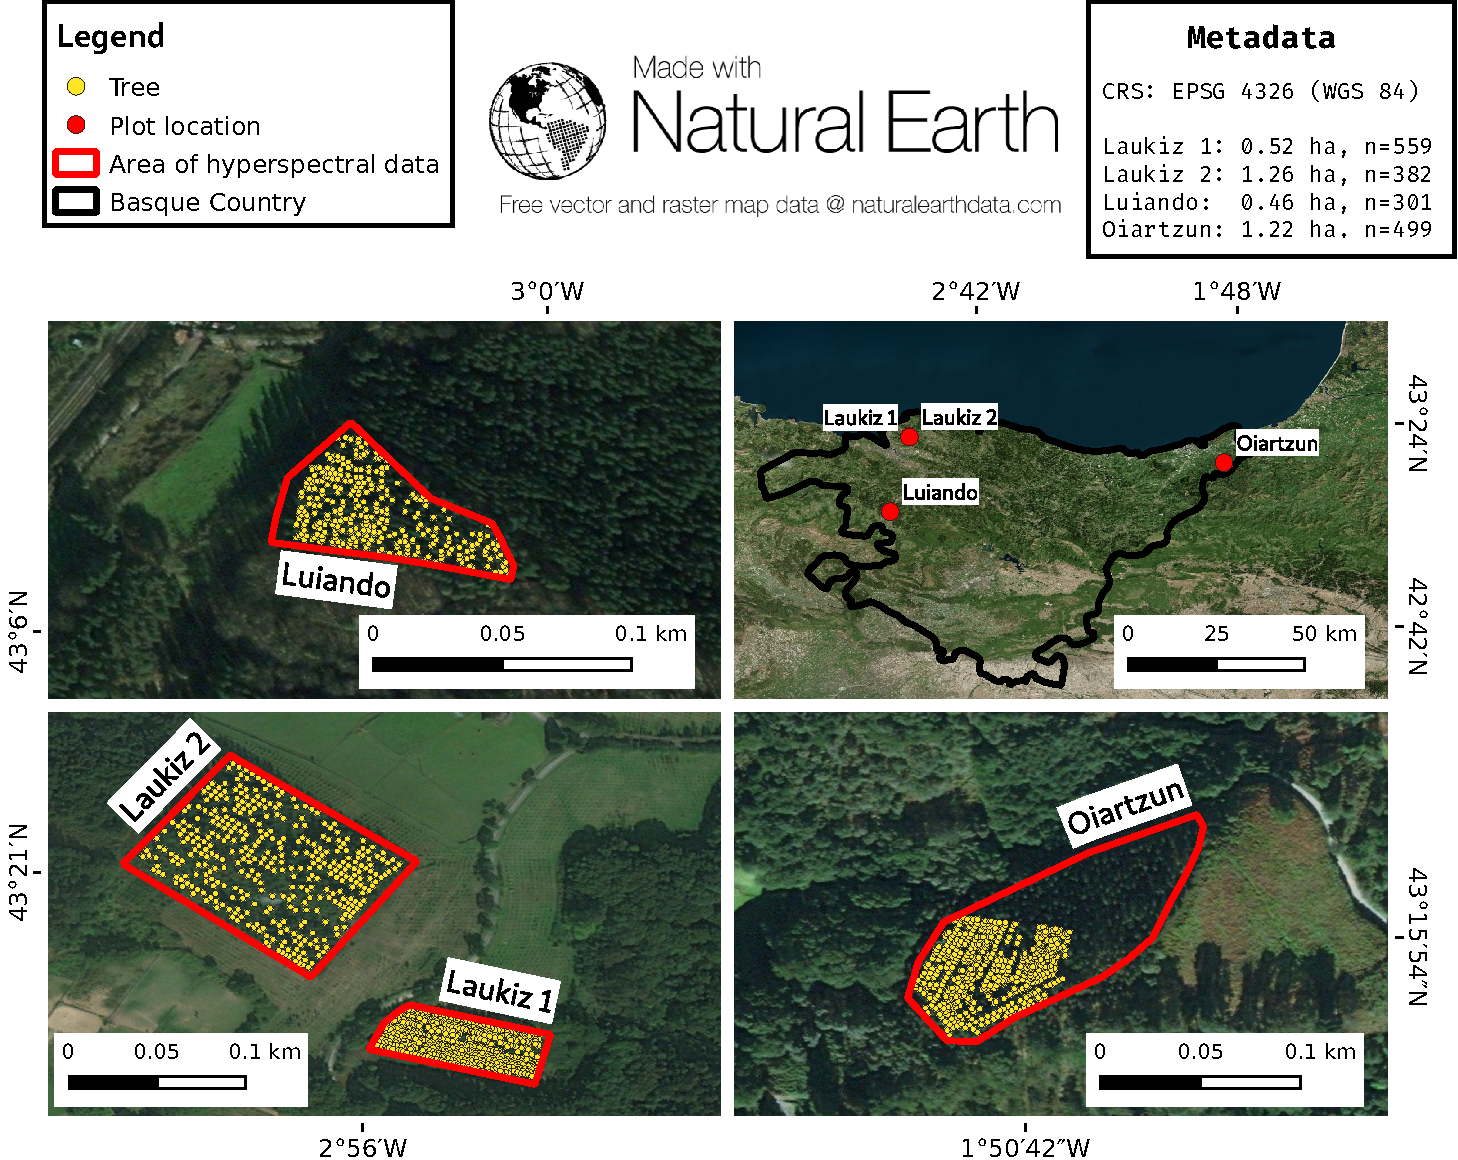
\includegraphics[width=\textwidth] {study_area_hyperspectral.pdf}}
		\caption{Information about the plot locations, the area of hyperspectral coverage and the number of trees per plot.}
		\label{fig:study_area}
	\end{center}
\end{figure}

\subsection{Hyperspectral data}

\noindent The airborne hyperspectral data was acquired during two flight campaigns on September 28th and October 5th 2016, both around 12 am.
The images were taken using a AISAEAGLE-II sensor.
All preprocessing steps (geometric, radiometric, atmospheric) have been conducted by the \ac{ICGC}.
The first four bands are corrupted, leaving 122 bands with valid information.
Additional metadata information is available in Table 1:

% parameter limits
\begin{table}[b!]
\centering
\caption[t]{Specifications of hyperspectral data.}
\begingroup\footnotesize
\begin{tabular}{ll}
	\\
	Characteristic         & Value                               \\
	\hline
	Geometric resolution   & 1 m                                 \\
	Radiometric resolution & 12 bit                              \\
	Spectral resolution    & 126 bands (404.08 nm - 996.31 nm)   \\
	Correction:            & Radiometric, geometric, atmospheric
\end{tabular}
\endgroup
\label{tab:hyperparameter_limits}
\end{table}

\section{Methods}

\noindent For all analysis steps we used the open-source statistical programming language R \citep{R_core}.
The algorithm implementations of the following packages have been used: \textit{xgboost} \citep{chenXGBoostScalableTree2016} (\textit{xgboost}), \textit{kernlab} \citep{kernlab} (Support Vector Machine) and \textit{glmnet} \citep{glmnet} (Ridge Regression).
We used the R package \textit{mlr} for all modeling related steps.
It provides a standardized interface for a wide variety of statistical and machine-learning models in R simplifying essential modeling tasks such as hyperparameter tuning, model performance evaluation and parallelization \citep{bischlMlrMachineLearning2016}.
We provide the complete code and required data as a Mendeley dataset to make this work fully reproducible [STILL TO COME].

\subsection{Derivation of indices}

\noindent To use the full information from the hyperspectral data, we calculated all possible vegetation indices that are available in the \textit{hsdar} package (90 in total) and all possible \ac{NRI} combinations.
We were interested if NRIs of arbitrary band combinations will have a substantial effect on the predictive power of the fitted model.
The NRIs were calculated using the following formula:

\begin{equation}
	NRI_{i,j} = \frac{b_{i} - b_{j}}{b_{i} + b_{j}}
\end{equation}

\noindent
where $i$ and $j$ are the respective band numbers.

\bigbreak

\noindent To account for geometric offsets (which were reported with up to 1 m from \ac{ICGC}), we used a buffer of two meters around the centroid of the respective tree.
The mean value of all pixels touched by the buffer was assigned as the final value of each index.
In total, $\frac{125*126}{2} = 7875$ NRIs were calculated .
Due to four corrupted bands and numerical problems for some band combinations, some indices returned \texttt{NA} for specific observations.
We removed all indices from the dataset that showed one or more \texttt{NA} values (across all plots) since we valued a single observation more than having an additional NRI as a predictor variable.
In total, 7471 indices had no \texttt{NA} values and were subsequently used as predictors.

\subsection{Benchmarking of algorithms}

\noindent Three algorithms (\textit{xgboost}, \textit{\ac{SVM}} and \textit{\ac{RR}}) were benchmarked on their predictive performance.
Besides the well-known \ac{SVM} algorithm \citep{Vapnik1998}, we also used \textit{xgboost} which is ensemble method relying on the idea of tree boosting that gained a lot of attention in recent years \citep{chenXGBoostScalableTree2016}.
We added penalized L2 (Ridge) regression to the portfolio due to its ability to handle highly correlated covariates \citep{hoerlRidgeRegressionBiased1970}.
One of the most popular machine-learning algorithm, Random Forest \citep{Breiman2001}, was not considered for this study: Due to the high number of variables, model fitting times in the range hours for a single model fit were not practicable for this work.
These high fitting times are caused by hyperparameter \texttt{mtry} which scales with the number of variables \citep{Probst2018b}.
After the selection of the best model, we checked if the winning algorithm can achieve a similar performance when using only the most important variables compared to using all variables.
A successful feature selection simplifies the spatial prediction task because the prediction dataset needs to consist of less variables.
Furthermore, model complexity and fitting times are reduced.

\subsubsection{Performance estimation}

\noindent The algorithms were benchmarked in two ways:

\begin{enumerate}
	\item Using spatial block \ac{CV} on the plot level with each plot serving as the test set once. Four performance estimates were retrieved, one for each fold.
	\item Using five-fold five-time repeated spatial \ac{CV} within each plot based on the k-means clustering approach of \cite{sperrorest} (\autoref{fig:spcv}).
\end{enumerate}

\noindent As we used the best algorithm of 1) for the spatial prediction, we first conducted the model selection on this setup and only applied the winning algorithm on 2).

\begin{figure} [t!]
	\begin{center}
		\makebox[\textwidth]{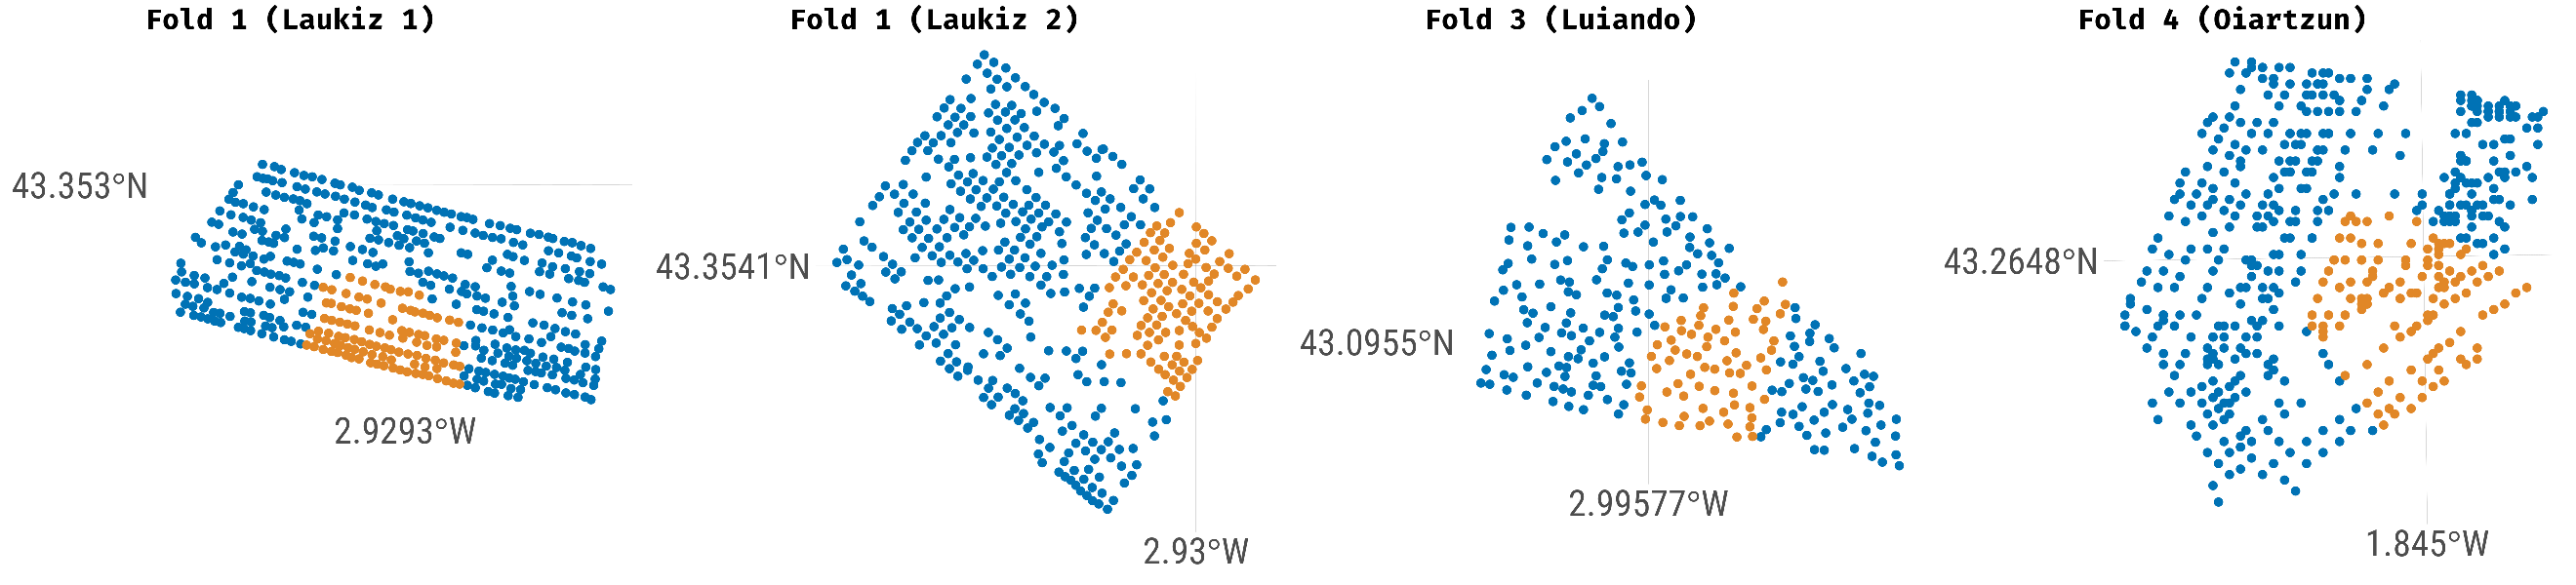
\includegraphics[width=1\textwidth] {spcv_folds_demon_plots.pdf}}
		\caption{Fold 1 of the spatial partitioning using k-means clustering for \textit{Laukiz 1}, \textit{Laukiz 2}, \textit{Luiando} and \textit{Oiartzun}.}
		\label{fig:spcv}
	\end{center}
\end{figure}

\subsubsection{Hyperparameter tuning}
\label{meth:smbo}

\noindent To tune the hyperparameters of the algorithms, we used \ac{SMBO} via the R package \textit{mlrMBO} \citep{mlrMBO}.
This Bayesian approach first composes \textit{n} randomly chosen hyperparameter settings out of a user defined search space.
After these \textit{n} tries have been evaluated, a new hyperparameter setting, which is going to be evaluated next, is proposed based on a fitted regression model.
The regression model estimates the performance of the machine-learning method for unknown hyperparameter settings.
Using these estimates, a new promising hyperparameter setting is proposed to be evaluated next.
This strategy continues until a termination criterion, defined by the user, is reached \citep{Hutter2011, Jones1998}.

In this work we used an initial design of 30 randomly composed hyperparameter settings and a termination criterion of 20 iterations, resulting in a total budget of 50 evaluated hyperparameter settings per fold.
The advantage of this tuning approach is that it substantially reduces the tuning budget which is needed to find a setting close to the global minimum compared to methods that do not use information from previous runs, such as random search or grid search \citep{Bergstra2012}.

\subsection{Variable importance}

\noindent To find indices that contributed most to model performance, we used the internal variable importance measure of the \textit{xgboost} algorithm.
This score is calculated by taking the contribution of each feature for each tree in the fitted model.
The higher the score of a variable, the more important it is for the fitted model when making predictions \citep{chenXGBoostScalableTree2016}.
The variable importance measure is automatically computed during model fit.
In contrast to other approaches such as permutation-based ones, the \textit{xgboost} score is composed out of three parts that contribute to the overall importance \citep{chenXGBoostScalableTree2016}:

\begin{itemize}
	\item Gain: The relative contribution of the feature to the model
	\item Cover metric: How often a feature was selected to be the deciding feature in a tree for a specific observation
	\item Frequency How often a feature occurs in all trees of the model
\end{itemize}

\noindent The \textit{Gain} features is the most important one among the three.
All measures sum up to one \citep{chenXGBoostScalableTree2016}.

% partial dependence plots??

\section{Results}

\subsection{Plot characteristics}

% defoliation boxplots
\begin{figure} [t!]
	\begin{center}
		\makebox[\textwidth]{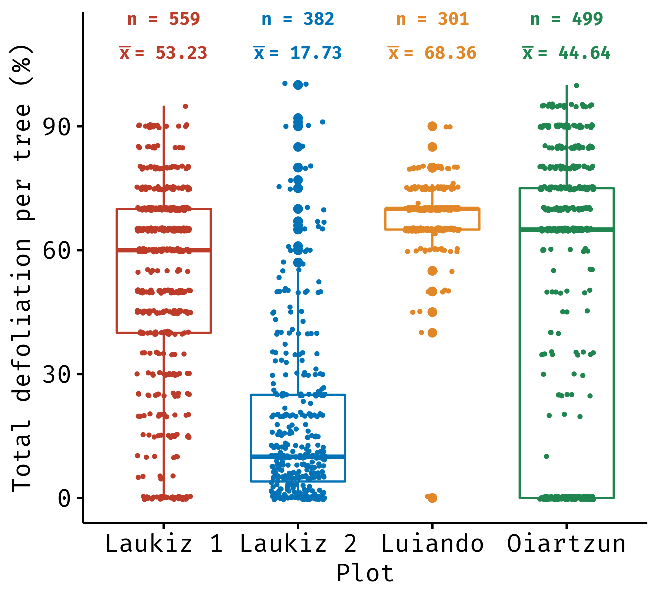
\includegraphics[width=0.7\textwidth] {boxplot_defol.pdf}}
		\caption{Descriptive statistics of the response variable \textit{defoliation}.}
		\label{fig:defol_boxplots}
	\end{center}
\end{figure}

\noindent \textit{Oiartzun} shows the highest defoliation ($\bar{x} = 69.22 \%$) among the plots while \textit{Laukiz 2} is the healthiest ($\bar{x} = 13.54 \%$) (\autoref{fig:defol_boxplots}).
All plots besides \textit{Luiando} show an evenly distributed level of defoliation across the entire plot.

\noindent The high degree of defoliation for \textit{Luiando} and \textit{Oiartzun} is also visible in the spectral signatures of the plots (\autoref{fig:spectral_signatures}).
Both plots show lower mean reflectance values around the wavelength range 800 nm - 1000 nm compared to \textit{Laukiz 1} and \textit{Laukiz 2}.
\textit{Oiartzun} is almost completely missing the reflectance drop at around 815 nm that is visible for all other plots but instead shows a higher magnitude for the reflectance increase at around 920 nm.

\noindent \textit{Laukiz 2} shows a mean tree density of 61.59 m (\autoref{fig:plot-characteristics}) while all other plots have a higher density (34.64 m (Laukiz 1), 33.01 m (Luiando), 34.96 m (Oiartzun)) (\autoref{fig:plot-characteristics}).

\subsection{Predictive performance}

% Performance estimates
\begin{table}[t!]
\centering
\caption[t]{Spatial block \ac{CV} performances of \textit{RR}, \textit{SVM} and \textit{xgboost} using \ac{RMSE} as the error measure.
	Mean and standard deviation are shown.}
\begingroup\footnotesize
\begin{tabular}{llll}
	RR            & SVM           & xgboost       & xgboost (7 variables) \\
	\hline
	59.10 (22.71) & 36.23 (15.73) & 33.26 (16.61) & 29.59   (16.09)       \\
	\bottomrule
\end{tabular}
\endgroup
\label{tab:model_comparison}
\end{table}

\begin{table}[b!]
\centering
\caption[t]{Predictive performance of \textit{xgboost} using all observations and all variables (All Observations/all variables), all observations and the seven most important variables only (All Observations/7 variables) and observations from specific plots only (Plot level observation/all variables) with \ac{RMSE} as the error measure. The performance estimates for "All Observations" correspond to the fold for which the respective plot was serving as the test set (block CV). Column "Plot level observations", shows the mean RMSE estimates at the repetition level of a five-fold five-time repeated spatial CV, scored by using data of the respective plot only.}
\begingroup\footnotesize
\begin{tabular}{llll}
	\\
	Plot/Data & \specialcell{All Observations/ \\{all variables (Block CV)}} & \specialcell{All Observations/         \\ {7 variables (Block CV)}} & \specialcell{Plot level observations/\\{all variables (SpCV)}} \\
	\hline
	Laukiz 1  & 22.03                                                                              & 21.47                          & 19.18 \\
	Laukiz 2  & 51.75                                                                              & 49.94                          & 17.24 \\
	Luiando   & 13.20                                                                              & 15.37                          & 8.30  \\
	Oiartzun  & 32.97                                                                              & 17.62                          & 14.40 \\
	\bottomrule
\end{tabular}
\endgroup
\label{tab:supermodel_performance}
\end{table}

\subsubsection{Algorithm benchmarking}

\noindent The \textit{xgboost} algorithm showed the lowest error (33.26 RMSE) when benchmarking the learners on the complete dataset of all plots (\autoref{tab:model_comparison}).
While the \textit{SVM} performance was only slightly worse (36.23 RMSE), \textit{RR} showed a substantially worse performance than \textit{xgboost} (59.10 RMSE).

\subsubsection{Single models vs. super model}

\noindent Comparing the mean predictive performance of models fitted at the plot level against the performance of the model that was fitted using all data (super model), the plot-level models showed a better performance in all cases (\autoref{tab:supermodel_performance}).
The highest difference between both datasets occurred for plot \textit{Laukiz 2} with a difference of 34.51 RMSE.

Using only the seven most important variables (\autoref{fig:var-imp}) for the super model showed small increases in performance for \textit{Laukiz 1} and \textit{Laukiz 2}, a small decrease for \textit{Luiando} and almost a reduction of 50\% of the error for \textit{Oiartzun} (32.97 vs. 17.62 RMSE) (\autoref{tab:supermodel_performance}).

\subsubsection{RMSE vs. plot characteristics}

\noindent An increase of the error rate was observed with an increase of descriptive plot measures such as mean point density and the coefficient of variation (based on the response variable \textit{defoliation}) (\autoref{fig:plot-characteristics}).

\begin{figure} [t!]
	\begin{center}
		\makebox[\textwidth]{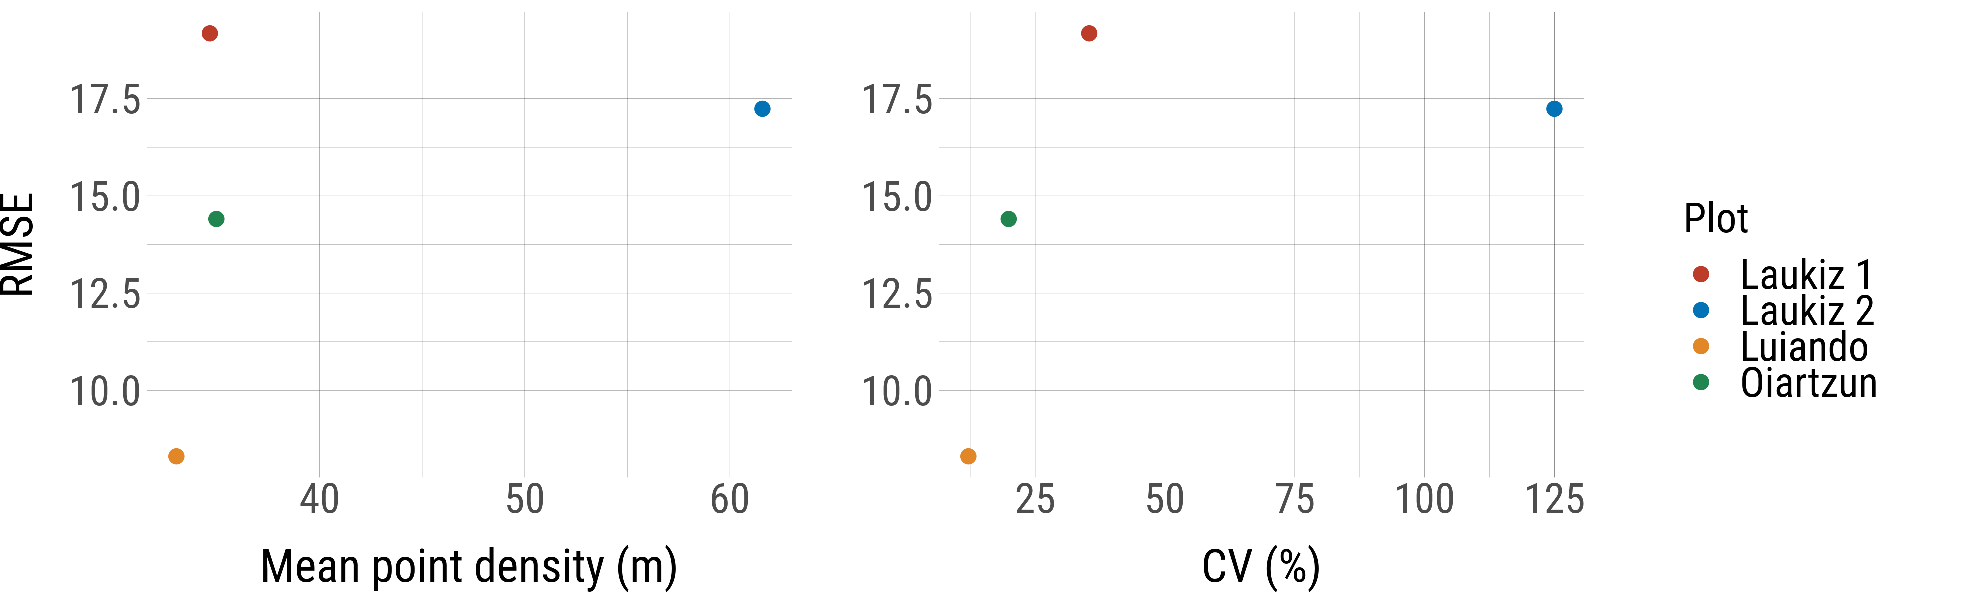
\includegraphics[width=\textwidth] {plot-characteristics.pdf}}
		\caption{RMSE vs. mean point density and coefficient of variation (defoliation).}
		\label{fig:plot-characteristics}
	\end{center}
\end{figure}

\subsection{Variable importance}

\noindent The seven most important features of the super model in this study were vegetation indices with the \textit{EVI} \citep{hueteComparisonVegetationIndices1997} being the most important one (\autoref{fig:var-imp}).

\begin{equation}
	EVI = 2.5*\frac{R_{800}-R_{670}}{R_{800}-(6*R_{670})-(7.5*R_{475})+1)}
\end{equation}

\noindent where $R$ = Reflectance at the respective wavelength.

\bigbreak

\noindent Vegetation index \textit{GDVI} appears three times among the first seven most important features (\autoref{fig:var-imp}) with different \texttt{n} values.
This is because it was computed four times, with \texttt{n} ranging from 1 - 4 \citep{wuEstimatingChlorophyllContent2008}:

\begin{equation}
	GDVI = \frac{R_{800}^n-R_{680}^n}{R_{800}^n+R_{680}^n}
\end{equation}

\bigbreak

\noindent The seven most important features (\textit{EVI}, \textit{GDVI\_4}, \textit{D1}, \textit{GDVI\_3}, \textit{GDVI\_2}, \textit{mNDVI} and \textit{mSR}) showed a substantial difference in the importance score compared to all following variables (\autoref{fig:var-imp}).

\begin{figure} [b!]
	\begin{center}
		\makebox[\textwidth]{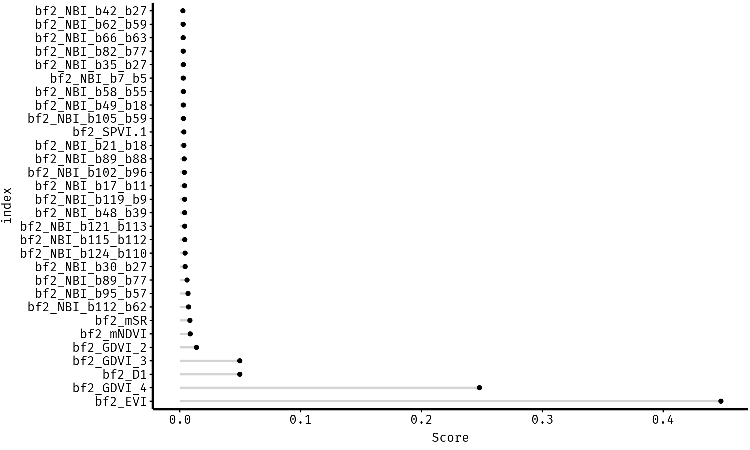
\includegraphics[width = 1\textwidth] {var-imp-xgboost.pdf}}
		\caption{The 30 most important variables as estimated by the internal variable importance measure of the \textit{xgboost} algorithm. The higher the score, the more important the feature.
			"bf2" notes that a buffer of 2 meter was used to extract the variable information to the tree observation. "NRI" means that a normalized ratio index with the subsequent bands was calculated. Features without "NRI" prefix are vegetation indices, e.g. "bf2\_EVI".}. %An overview of the vegetation indices can be found \href{https://rdrr.io/cran/hsdar/man/vegindex.html}{here}.}
		\label{fig:var-imp}
	\end{center}
\end{figure}

\begin{table}[t!]
\centering
\caption[t]{Formulas of the five most important vegetation indices of the super model. $R$ = Reflectance at wavelength, $D$ = First derivation of reflectance value at wavelength.}
\begingroup\footnotesize
\begin{tabular}{llll}
	\\
	Acronym & Name                      & Formula                                                            & Reference                                                 \\
	\hline
	EVI     & Enhanced vegetation index & $2.5*\frac{R_{800}-R_{670}}{R_{800}-(6*R_{670})-(7.5*R_{475})+1)}$ & \cite{hueteComparisonVegetationIndices1997}               \\
	GDVI    & Generalized DVI*          & $\frac{R_{800}^n-R_{680}^n}{R_{800}^n+R_{680}^n}$                  & \cite{wuEstimatingChlorophyllContent2008}                 \\
	D1      & Derivative Index          & $\frac{D_{730}}{D_{706}}$                                          & \cite{zarco-tejadaSteadystateChlorophyllFluorescence2003} \\
	mNDVI   & Normalized DVI*           & $  \frac{R_{800}-R_{680}}{(R_{800}+R_{680}-2*R_{445}}$             & \cite{simsRelationshipsLeafPigment2002}                   \\
	mSR     & Simple Ratio Index        & $\frac{R_{800}-R_{445}}{R_{680}-R_{445}}$                          & \cite{simsRelationshipsLeafPigment2002}                   \\
	\bottomrule
	\multicolumn{2}{l}{\small{* Difference Vegetation Index}}
\end{tabular}
\endgroup
\label{tab:most_imp_vars}
\end{table}

\noindent The best NRI scored rank eight (band 112 and band 62).
All further places up to rank 30 were occupied by NRIs.

\subsection{Spatial prediction}

\begin{figure} [b!]
	\begin{center}
		\makebox[\textwidth]{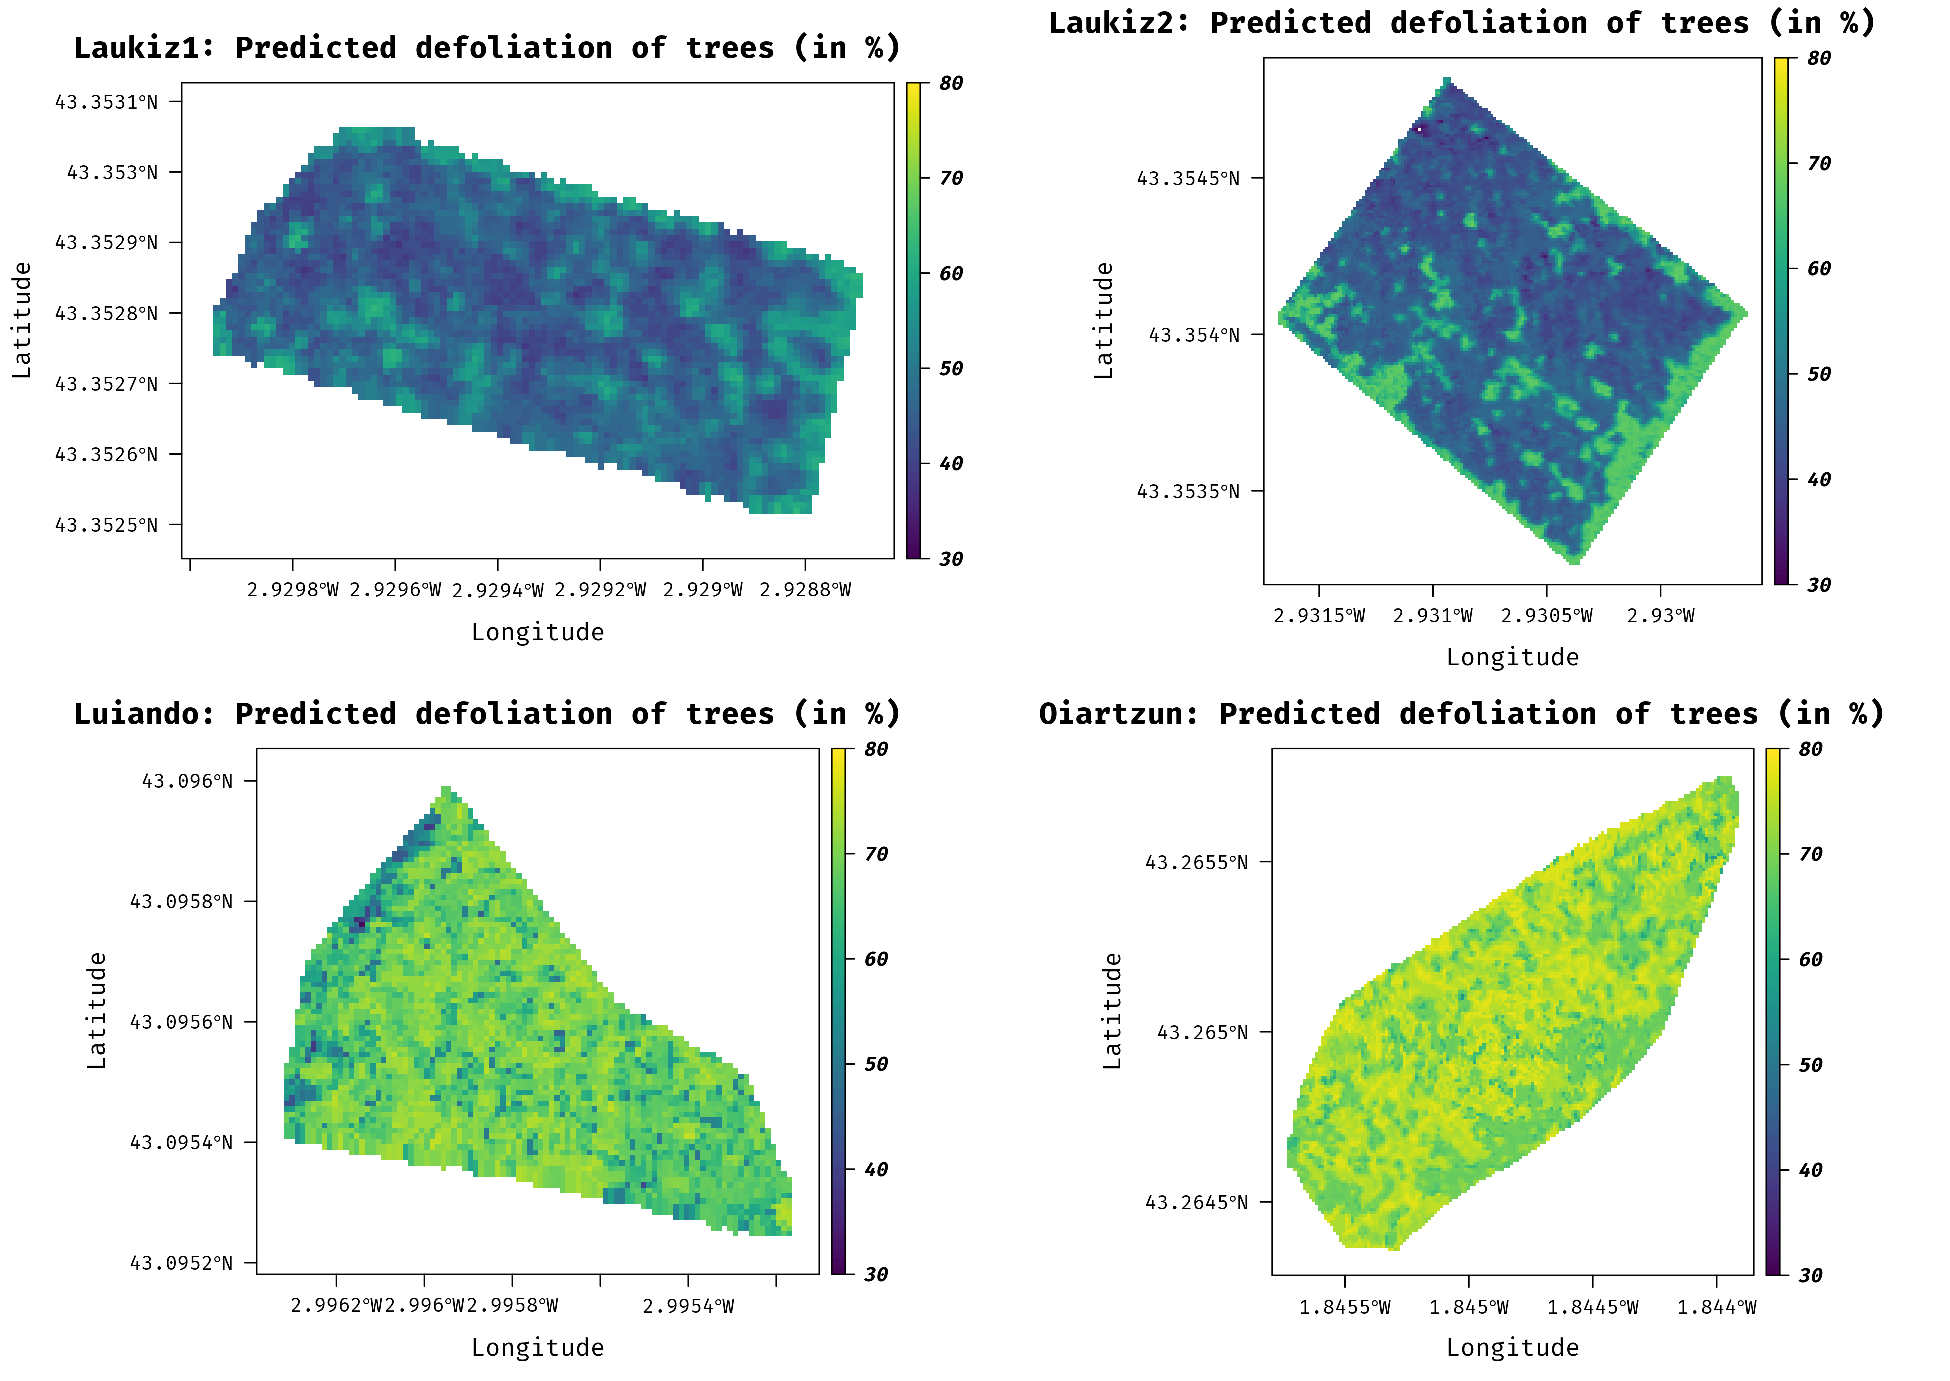
\includegraphics[width = 1\textwidth] {predictions_demon_plots.pdf}}
		\caption{Spatially predicted defoliation (in \%) from \textit{xgboost} of \textit{Laukiz 1}, \textit{Laukiz 2}, \textit{Luiando} and \textit{Oiartzun}.}
		\label{fig:pred_demon_plots}
	\end{center}
\end{figure}

\begin{figure} [t!]
	\begin{center}
		\makebox[\textwidth]{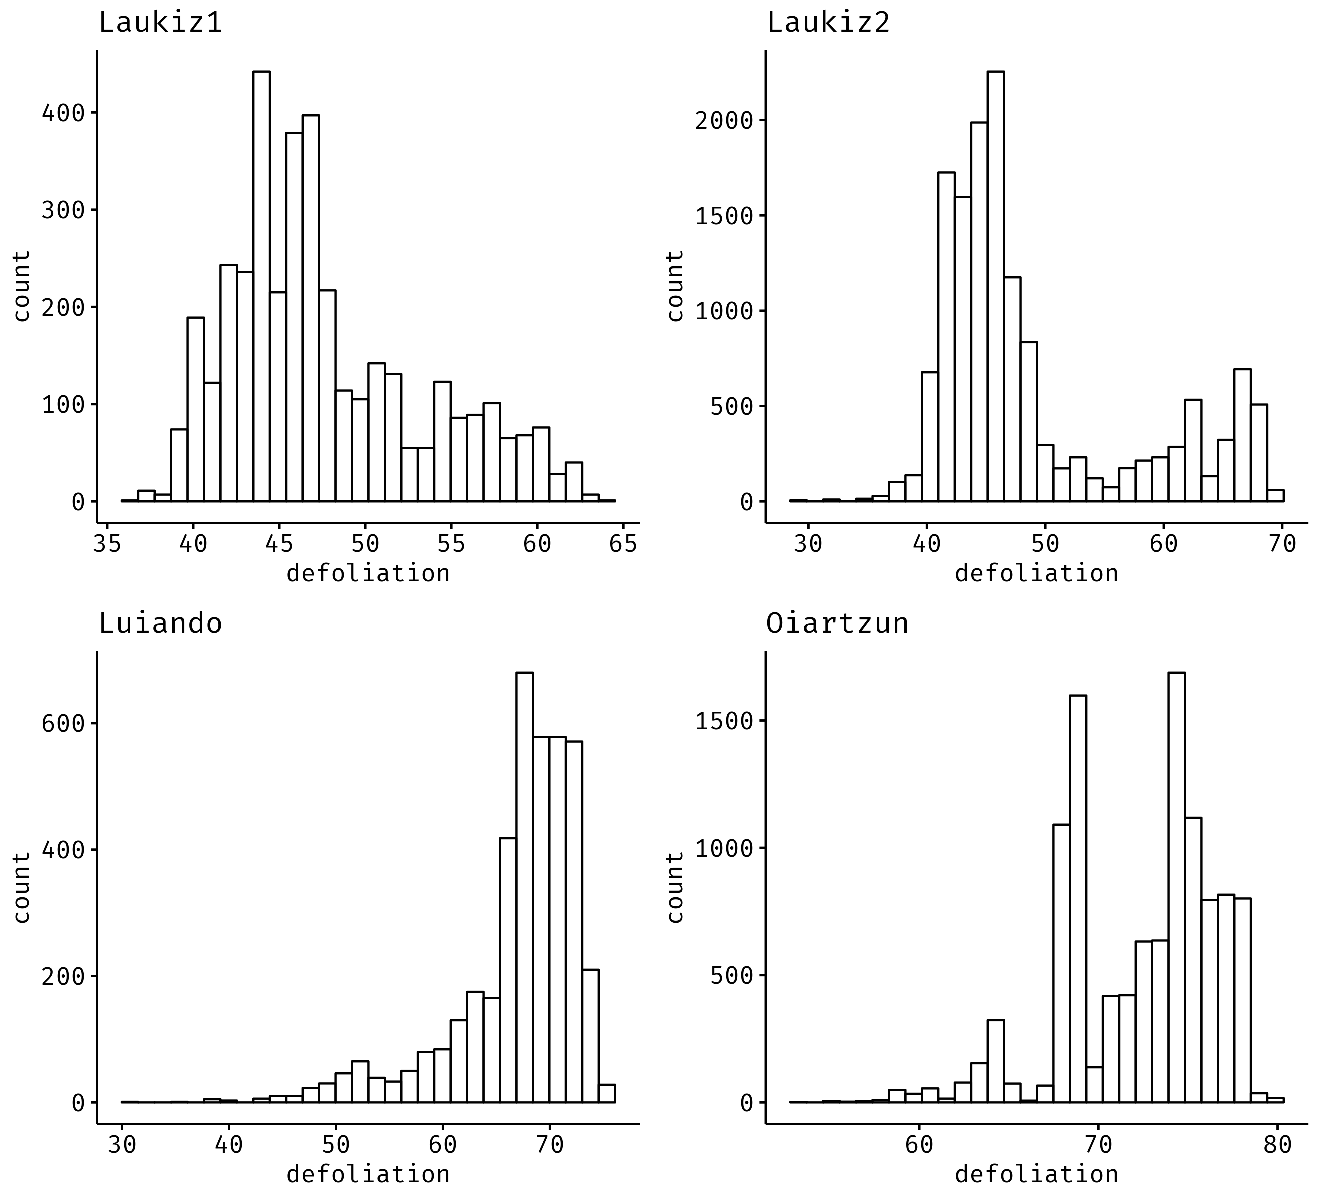
\includegraphics[width = 0.6\textwidth] {predictions_demon_plots_hists.pdf}}
		\caption{Histograms of predicted defoliation (in \%) from \textit{xgboost} of \textit{Laukiz 1}, \textit{Laukiz 2}, \textit{Luiando} and \textit{Oiartzun}.}
		\label{fig:pred_demon_plots_hists}
	\end{center}
\end{figure}

\noindent The plots with a higher mean defoliation (\textit{Luiando} and \textit{Oiartzun}) showed a good visual separability compared to the healthier plots \textit{Laukiz 1} and \textit{Laukiz 2} (\autoref{fig:pred_demon_plots}).
All predicted values ranged between 30 \% and 80 \% defoliation with \textit{Luiando} showing the smallest variance (\autoref{fig:pred_demon_plots_hists}).

The high error of the super model for \textit{Laukiz 2} (49.94 RMSE) is also visible in the respective histogram as most predictions range between a defoliation of 40 \% - 50 \% (\autoref{fig:pred_demon_plots_hists}) while in fact most trees of \textit{Laukiz 2} show an actual defoliation of around 20 \% (\autoref{fig:defol_boxplots}).

For the less defoliated plots \textit{Laukiz 1} and \textit{Laukiz 2} a subtle level of separation between trees and bare ground is visible (\autoref{fig:pred_demon_plots}).
This is not the case for the other two higher defoliated plots for which bare ground and defoliated predictions are mainly in the same value range (around 60 \% - 80 \%).

\section{Discussion}

\subsection{Derivation of indices}

\noindent The buffer of 2 m that we used to generate the index value for each observation can be seen critical.
When using no buffer at all, the possibility is high that a pixel value gets assigned to the tree observation that does not spatially match (due to the geometric offset of 1 m in the hyperspectral data).
Using a buffer of more than 2 meters would increase the probability of merging information from other trees into the pixel value, blurring the actual value of the tree observation.
Thats why in our view using a buffer of 2 m was the best compromise here.

another critical point is that the exact number of contributing pixels to the final index value of an observation cannot be determined as it depends on the location of the tree within the pixel grid.
As the buffer is a circle, it depends on the exact location of a tree observation within a pixel how much surrounding pixels are touched by the buffer.
If a tree observation is located at the border of the plot, some directions of the buffer will contain no values and the subsequent index value will be calculated using less pixels than if the tree observation is located in the middle of the plot.

All these points introduced a bias of an unknown magnitude into the data.
This has to be considered when making interpretations about the outcome of this study.

\subsection{RMSE vs. plot characteristics}

\noindent Relating the modeling error to plot characteristics (mean point density, coefficient of variation) did not show a clear picture: For both comparisons, \textit{Laukiz 2} did not follow the pattern that was observed from the other three plots (\autoref{fig:plot-characteristics}) of having an increase in error with an increase in mean point density and coefficient of variation.

It needs to be considered that we only looked at four plots in this work.
To make a robust statement about a possible relationship between modeling error and plot characteristics, a larger sample size of plots is needed. 

\subsection{Predictive Performance}

\subsubsection{Algorithm benchmarking}

\noindent The relatively large difference in performance between \textit{RR} (59.10 RMSE) and the machine-learning models (36.23 and 33.26 RMSE) is remarkable.
\textit{RR} has shown promising results in other studies when many highly-correlated predictors were involved \citep{hernandezUsingRidgeRegression2015, imaniRidgeRegressionbasedFeature2015}.
However, in this study, \textit{RR} was not able to achieve a sufficient performance score compared to \textit{SVM} and \textit{xgboost} even though its hyperparameter $\lambda$ was properly tuned using SMBO (\autoref{meth:smbo}).

While \textit{xgboost} showed a slightly better performance than \textit{SVM}, the latter has the advantage of only having two hyperparameters that need to be tuned.
This results in a shorter runtime.
Nevertheless, \textit{xgboost} showed the best performance and was subsequently selected to fit the models on the plot level and for the spatial prediction.

An important point that needs to be considered when interpreting the performance results is that we only related defoliation to indices derived from remote sensing data.
Possible other local variables that could help in predicting defoliation were not considered.
One example here is tree age: The older a tree the more vulnerable it may be to pathogen infections causing defoliation.
However, such predictors would not be available for a spatial prediction scenario and one of the main goals of this study is to relate defoliation to variables that are available on a larger scale (e.g. remote sensing indices).

\subsubsection{Single models vs. super model}

\noindent It is expected that models that were trained using observations from the respective plot only only achieve a better performance than the super model which was trained on observations from multiple plots (\autoref{tab:supermodel_performance}).
The low performance on \textit{Laukiz 2} for the super model is most likely due to the difference of this plot to all others: The fitted model on \textit{Laukiz 1}, \textit{Luiando} and \textit{Oiartzun} is not capable of reaching a good performance when \textit{Laukiz 2} is the evaluation dataset.
This is not surprising as \textit{Laukiz 2} shows substantially different plot characteristics compared to all others plots in terms of the distribution of the response variable \textit{defoliation} (\autoref{fig:defol_boxplots}) and the mean point density of trees (\autoref{fig:plot-characteristics}).

The low error for Luiando (8.30 RMSE) for the plot model validates the approach of relating defoliation to vegetation indices and NRIs.
The overall error of the super model (33.26 RSME) is expected to decrease if more plots would be available for training.
However, even if the fitted model would include at least one instance of every plot showing unique characteristics (e.g. here \textit{Laukiz 2} is substantially different to the others), the overall error would not become smaller than the error achieved when using data from the respective plot only.

An interesting find is that the model with only seven variables shows a better overall performance than the model with all 7471 variables (\autoref{tab:supermodel_performance}).
This leads to the conclusion that adding as many variables as possible to a model will not necessarily improve its performance but instead add noise to the model.
Too much information can be problematic for a model as it will have a hard time distinguishing between noise and important information in the variables \citep{liFeatureSelectionData2017, guyonIntroductionVariableFeature2003}.
However, to find the most important variables in the first place and to check for the performance difference, a model with all variables needs to fitted first.
Using a model with only a few predictors does not only simplify prediction tasks but also reduces runtime for hyperparameter tuning and performance estimation \citep{liuComputationalMethodsFeature2007}.

\subsection{Variable importance}

\noindent There are some downsides using the internal variable importance approach of \textit{xgboost}: Due to the contribution of three different parts to the overall importance score it is complicated to understand why a specific feature was selected.
Furthermore the importance calculation approach is only valid for this algorithm and cannot be compared to others.
Nevertheless, as we only relied on the variable importance for this specific algorithm, using the internal \textit{xgboost} approach was sufficient for this work.

It is expected that vegetation indices are most important for the model as these are most sensitive to changes in vegetation health \citep{croftApplicabilityEmpiricalVegetation2014}.
Even though we are not directly looking at vegetation health but using the level of defoliation as a proxy for tree health, vegetation indices were most important for the fitted model of this study (\autoref{fig:var-imp}).

\noindent Vegetation indices can help assessing defoliation in two ways:

\begin{itemize}
	\item Trees that show a high level of defoliation do also reflect their bad health status through the remaining foliation.
	\item Defoliated trees have more influence of bare ground information in their pixel values and will therefore be classified as defoliated by the model.
\end{itemize}

\noindent Even though no NRI made it among the most important variables in this study (\autoref{fig:var-imp}) (stating that the first seven of this study are the most important ones), it is notable that all ranks from 8 - 30 are occupied by NRI (\autoref{fig:var-imp}).
However, their relative importance was very small compared to the first seven ranks.

Restricting the important indices of this study to the first seven ranks can be seen critical as we only based the selection on a visual inspection of the variable importance results (\autoref{fig:var-imp}).
The decision to make a cut between rank seven and eight was based on a combination of two facts:

\begin{itemize}
	\item Using only vegetation indices is easier for large scale predictions using satellites like Sentinel-2 (most NRIs cannot be used with it because the spectral bands do not exist).
	\item The drop in the importance score of the variable importance results (\autoref{fig:var-imp}).
\end{itemize}

\noindent However, based on these two points, we could also have made the cut between rank five and 6 but including the two vegetation indices at rank six and seven will eventually improve the model and does not increase runtime.

\subsection{Spatial prediction}

\noindent The spatial predictions showed that the model tries to avoid making extreme predictions since most values ranged between a defoliation of 30 \% and 80 \%.
This behavior is mainly triggered by overfitting on the observations of the \textit{Laukiz 1}, \textit{Luiando} and \textit{Oiartzun} training plots.
The overfit then causes a high prediction error for \textit{Laukiz 2} for which a lot of defoliation values actually range between 0 \% and 20 \%.
The fitted model would need more training samples of plots with an unusual defoliation distribution to become more robust and achieve a better overall performance.

\subsection{Comparison to other studies}

\noindent Other studies analyzing defoliation found that reflectance differences between defoliated and 30 \% defoliated trees of up to 10\% exist in the \ac{NIR} region \citep{rengarajanModelingForestDefoliation2016}.
This corresponds with the finding of this study that the most important variables are located in the NIR region.

\cite{goodbodyDigitalAerialPhotogrammetry2018} used NDVI and structural measures in as inputs for a partial least squares analysis to model defoliation caused by the spruce budworm.
Results showed that metrics from spectral features were most important.
Incorporating spectral metrics could be a possible enhancement for future studies.

\cite{townsendGeneralLandsatModel2012} used Landsat data to model defoliation caused by insect herbivores.
They found that the \ac{NDII} ($\frac{Band 4 - Band 5}{Band 4 + Band 5}$) and the moisture stress index ($\frac{Band 5}{Band 4}$) gave better results than using NDVI.
Overall, they used 10 vegetation indices derived from Landsat data.

MODIS data was used by \cite{debeursEstimatingEffectGypsy2008} to model defoliation caused by the gypsy moth using vegetation indices such as NDVI, EVI, NDWI and NDII.

All of these examples validate the approach of using vegetation indices to model defoliation.
Even though the spatial resolution of the data in these studies varied between hundreds of meters (MODIS) \cite{debeursEstimatingEffectGypsy2008} and centimeters \cite{goodbodyDigitalAerialPhotogrammetry2018}, high resolution data is preferred to fit accurate models.
Also, the importance of certain indices (e.g. NDVI, EVI) will vary based on the data and resolution.
The finding of this work that the vegetation indices GDVI and EVI are most important for the fitted model could not be verified by other studies.
However, the presented ones did often only use a small subset of the vegetation indices that were used in this study.

We could not find a study that used recent machine-learning techniques in combination with a high amount of variables to model defoliation.
This fact highlights the importance of this work and will hopefully encourage scientists to use machine-learning techniques, feature selection methods and a wider selection of vegetation indices when assessing defoliation in the future.

\section{Conclusion}

\noindent In this work we used various indices derived from hyperspectral remote sensing data to estimate defoliationas a proxy for tree health in northern Spain.
In the algorithm comparison \textit{xgboost} showed the best performance among the tested ones.
Even though \ac{RR} is able to handle highly correlated data, it was far from achieving an acceptable performance in this work.

The fitted models on the plot level showed a promising performance with RMSE values between 8 and 20 which validated the approach of relating defoliation to remote sensing indices.
The performance of the model containing all data (four plots) was acceptable (RMSE 29.59) but can be improved by adding more observations from other plots in future studies.

The spatial prediction showed a satisfying result making it possible to distinguish highly defoliated plots from plots with low defoliation easily.
The most important indices for the fitted model were widely known vegetations indices such as EVI, GDVI or NDVI.
In future studies it would be interesting to link the indices of this work to other indicators of forest/vegetation health and analyze their importance and the model performances.

\section{Appendix}

\appendix
% https://tex.stackexchange.com/questions/248704/cross-reference-to-appendix-sections-in-elsarticle-document-class
\gdef\thesection{\Alph{section}} % corrected redefinition of "\thesection"
\makeatletter
\renewcommand\@seccntformat[1]{Appendix \csname the#1\endcsname.\hspace{0.5em}}
\makeatother

\section{Spectral signatures of each plot}

% spectral signatures
\begin{figure} [H]
	\begin{center}
		\makebox[\textwidth]{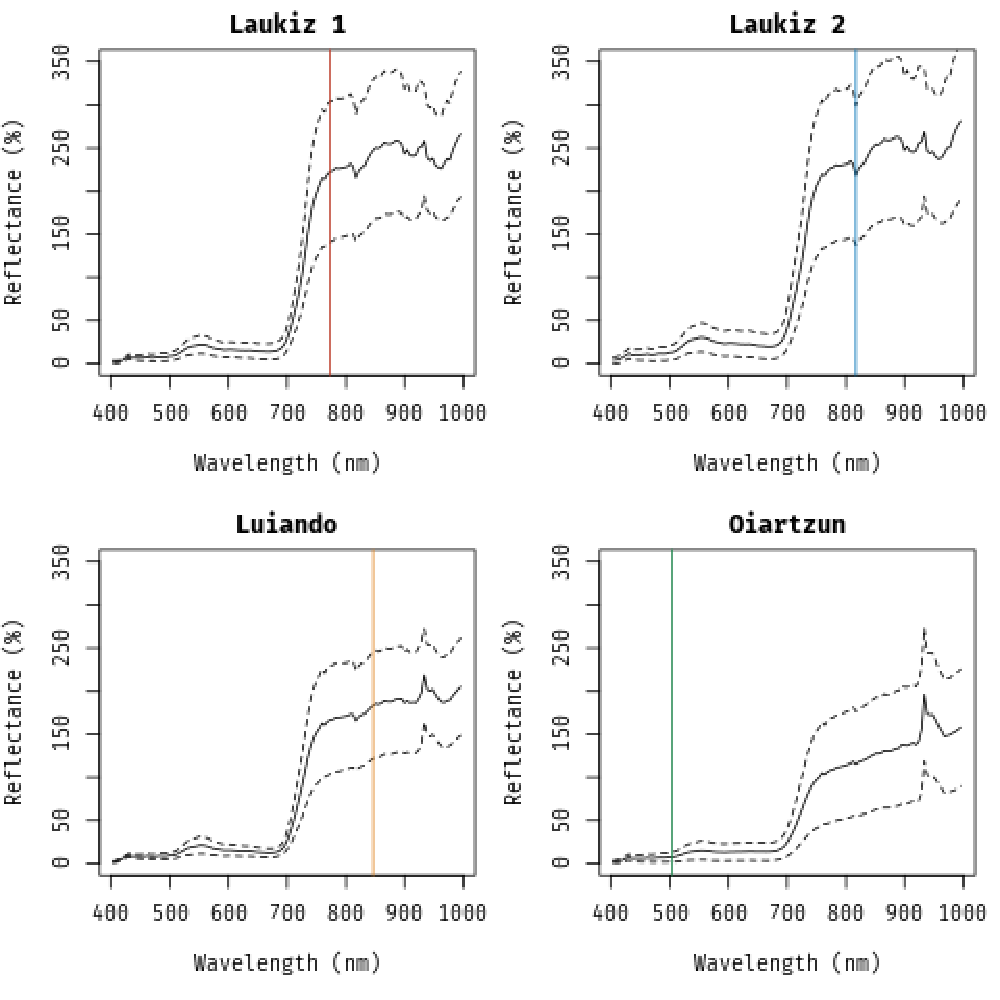
\includegraphics[width=\textwidth] {spectral_signatures.pdf}}
		\caption{Spectral signatures (mean and standard deviation) of each plot.}
		\label{fig:spectral_signatures}
	\end{center}
\end{figure}

\pagebreak

\section*{References}

\bibliography{Biblio_hyperspectral}

\end{document}
